%%%%%%%%%%%%%%%%%%%%
%
% $Beschreibung: Einleitung in das Projekt Demonstrator für einen Schrittmotor $
% $Autor: Grönke $
% $Datum: 09.06.2024 $
% $Pfad: DemonstratorSchrittmotor/DeveloperDoc/Contents/de/Projektbeschreibung.tex $
% $Version: 2 $
%
%
%%%%%%%%%%%%%%%%%%%


\chapter{Projektbeschreibung}

\section{Kurzbeschreibung des Demonstrators}

Ein Riemen wird von einem Schrittmotor angetrieben. An diesem Riemen ist ein Schlitten befestigt, der durch die Bewegung des Schrittmotors auf einer Linearführung bewegt wird. Am Gehäuse befindet sich ein Drehschalter, mit dem eine von zehn Bewegungsstufen ausgewählt werden kann. Nach der Auswahl kann das Programm mit der grünen Start/Stop-Taste gestartet werden. Die Status-LED leuchtet rot, sobald das Gerät betriebsbereit ist. Für die Referenzfahrt ist am Schrittmotorhalter ein Endschalter angebracht, damit der Schrittmotor auf eine definierte Position referenzieren kann. Es gibt zehn verschiedene Bewegungsstufen. Die Bewegungsstufen unterscheiden sich in der Geschwindigkeit. Mit jeder Stufe erhöht sich die Geschwindigkeit.

\section{Herausforderungen} 

Das Projekt kann in drei verschiedene Teilprojekte unterteilt werden, die zur Erfüllung der Aufgabe führen. Das erste ist der Aufbau des Demonstrators und die Auswahl der dafür notwendigen Hardwarekomponenten. Die Vorgabe war, den Aufbau nicht zu komplex zu gestalten und sich auf die wesentlichen Teile zu konzentrieren. Des Weiteren ist die Arbeit mit der Arduino IDE und die Programmierung des Arduino ein weiterer Teil. Der letzte Punkt ist der Umgang mit den elektronischen Bauteilen. Der Umgang mit den elektronischen Bauteilen muss sehr vorsichtig erfolgen, damit diese nicht durch den elektrischen Strom beschädigt werden.

\section{Lösungsansatz}

Durch die Erarbeitung der Herausforderungen können Lösungsansätze entwickelt werden. Im Vorfeld wurde eine erste Konzeptskizze erstellt, aus der Ideen entstanden. Im ersten Konzept sollte der Schrittmotor über einen Riementrieb eine Plattform axial bewegen, erkennbar in Abbildung \ref{ErsteKonzeptskizze}. Dabei sollte der Verfahrweg der Plattform über einen Abstandssensor mit einem vorgegebenen Abstand zu einem Objekt geregelt werden. Bewegt sich das Objekt auf den Abstandssensor zu oder von diesem weg, so bewegt sich die Plattform um einen definierten Abstand mit. Alle vorhandenen Bauteile sollen an einem Aluminiumprofil befestigt werden.

\begin{figure}[htb]
	\begin{center}
		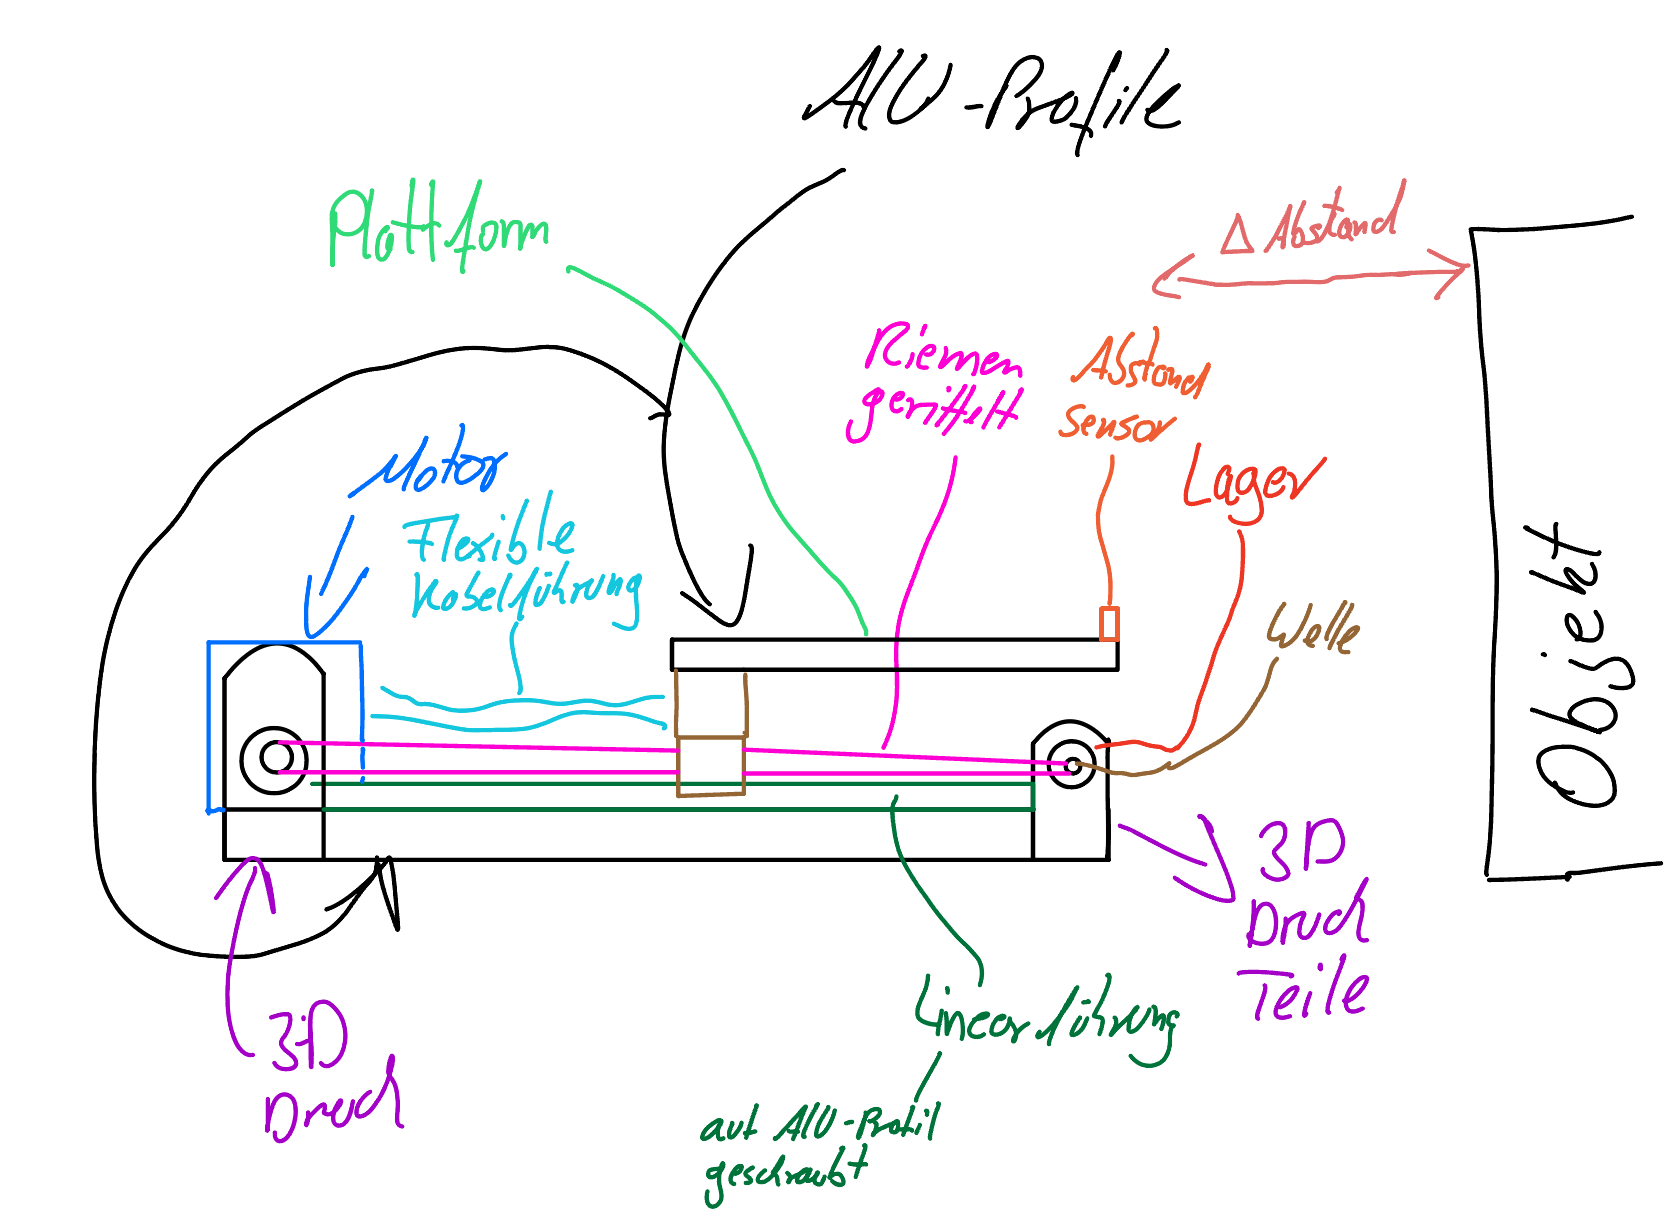
\includegraphics[width=\textwidth]{Images/Konzeptskizze1.png}
		\caption{Erste Konzeptskizze (Eigenaufnahme)} \label{ErsteKonzeptskizze}
\end{center}
\end{figure}  

Aufgrund der hohen Komplexität wurde beim zweiten Konzept, wie in Abbildung \ref{ZweiteKonzeptskizze} dargestellt, auf die Plattform inklusive Abstandssensor verzichtet. Stattdessen ist auf dem Schlitten der Linearführung ein Zeiger und auf dem Aluminiumprofil ein Lineal integriert. Der Schrittmotor soll über verschiedene Stufen unterschiedliche Bewegungsprofile demonstrieren. Insbesondere soll die Positioniergenauigkeit mit dem Zeiger dargestellt werden. Des Weiteren wurde ein Netzteil integriert, das sowohl den Motor als auch den Arduino mit Spannung versorgt. Weiterhin sind ein Schalter zum Ein- und Ausschalten des Demonstrators, ein Stufenschalter zur Auswahl der Stufen sowie ein Taster zum Starten des Demonstratorablaufs integriert.

\begin{figure}[H]
	\begin{center}
		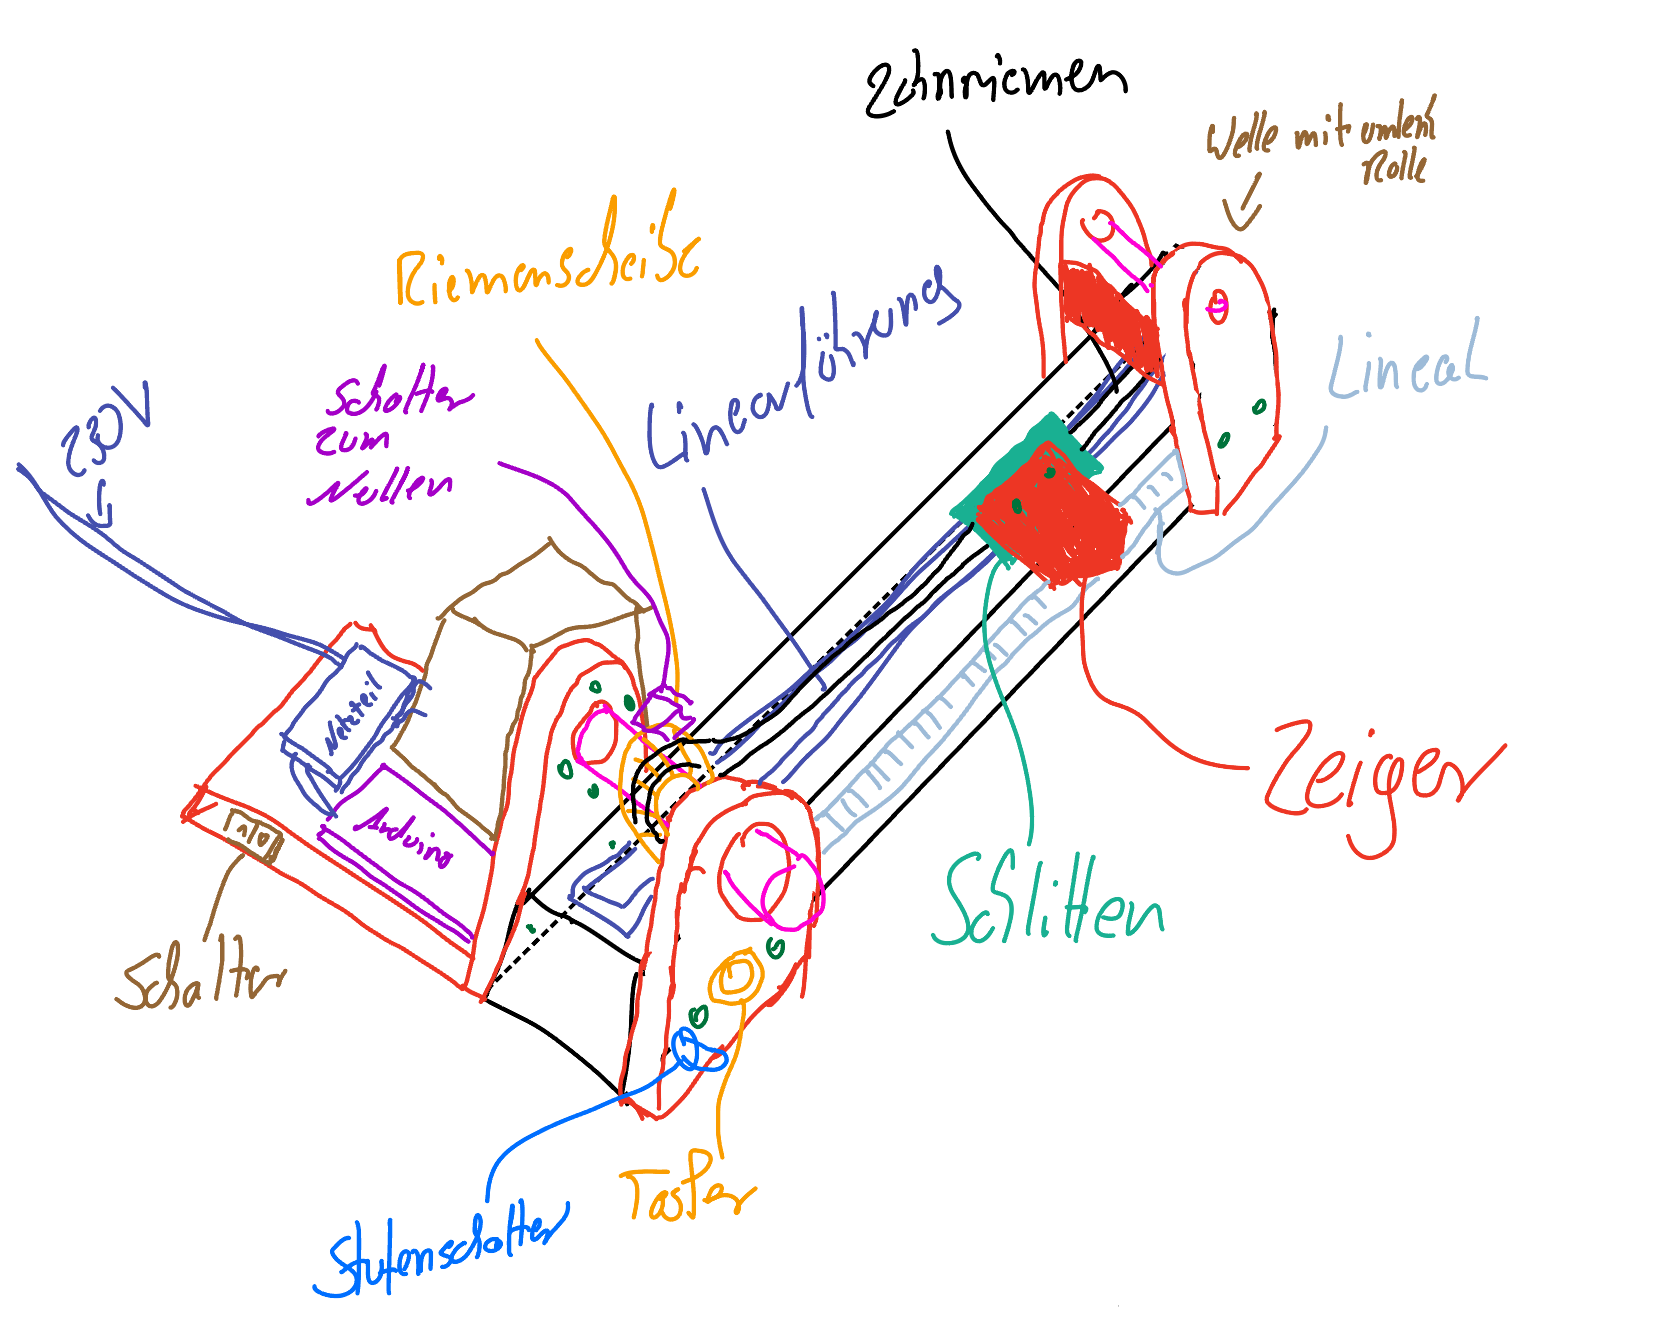
\includegraphics[width=\textwidth]{Images/Konzeptskizze2.png}
		\caption{Zweite Konzeptskizze (Eigenaufnahme)} \label{ZweiteKonzeptskizze}
	\end{center}
\end{figure}

Das zweite Konzept gefiel und wurde weiter ausgearbeitet, so dass mit dem Handbuch begonnen werden konnte (siehe Handbuch Demonstrator für einen Schrittmotor). In diesem Handbuch sollten vor allem die einzelnen Funktionen und die Bedienung aus Kundensicht geklärt werden. Parallel dazu konnte ein CAD-Modell erstellt werden, zu sehen in Abbildung \Ref{CADMOD}. Dazu konnte im Team eine MindMap erstellt werden, die alle möglichen Inhalte und zu erledigenden Aufgaben zusammenfasst, zu sehen in Abbildung \ref{Mindmap}. Im Vergleich zum zweiten Konzept wurde die Hardware aus Transportgründen auf das Aluminiumprofil gelegt und erhielt zum Schutz ein Gehäuse. Außerdem konnte eine Materialliste erstellt werden.

\begin{figure}[H]
	\begin{center}
		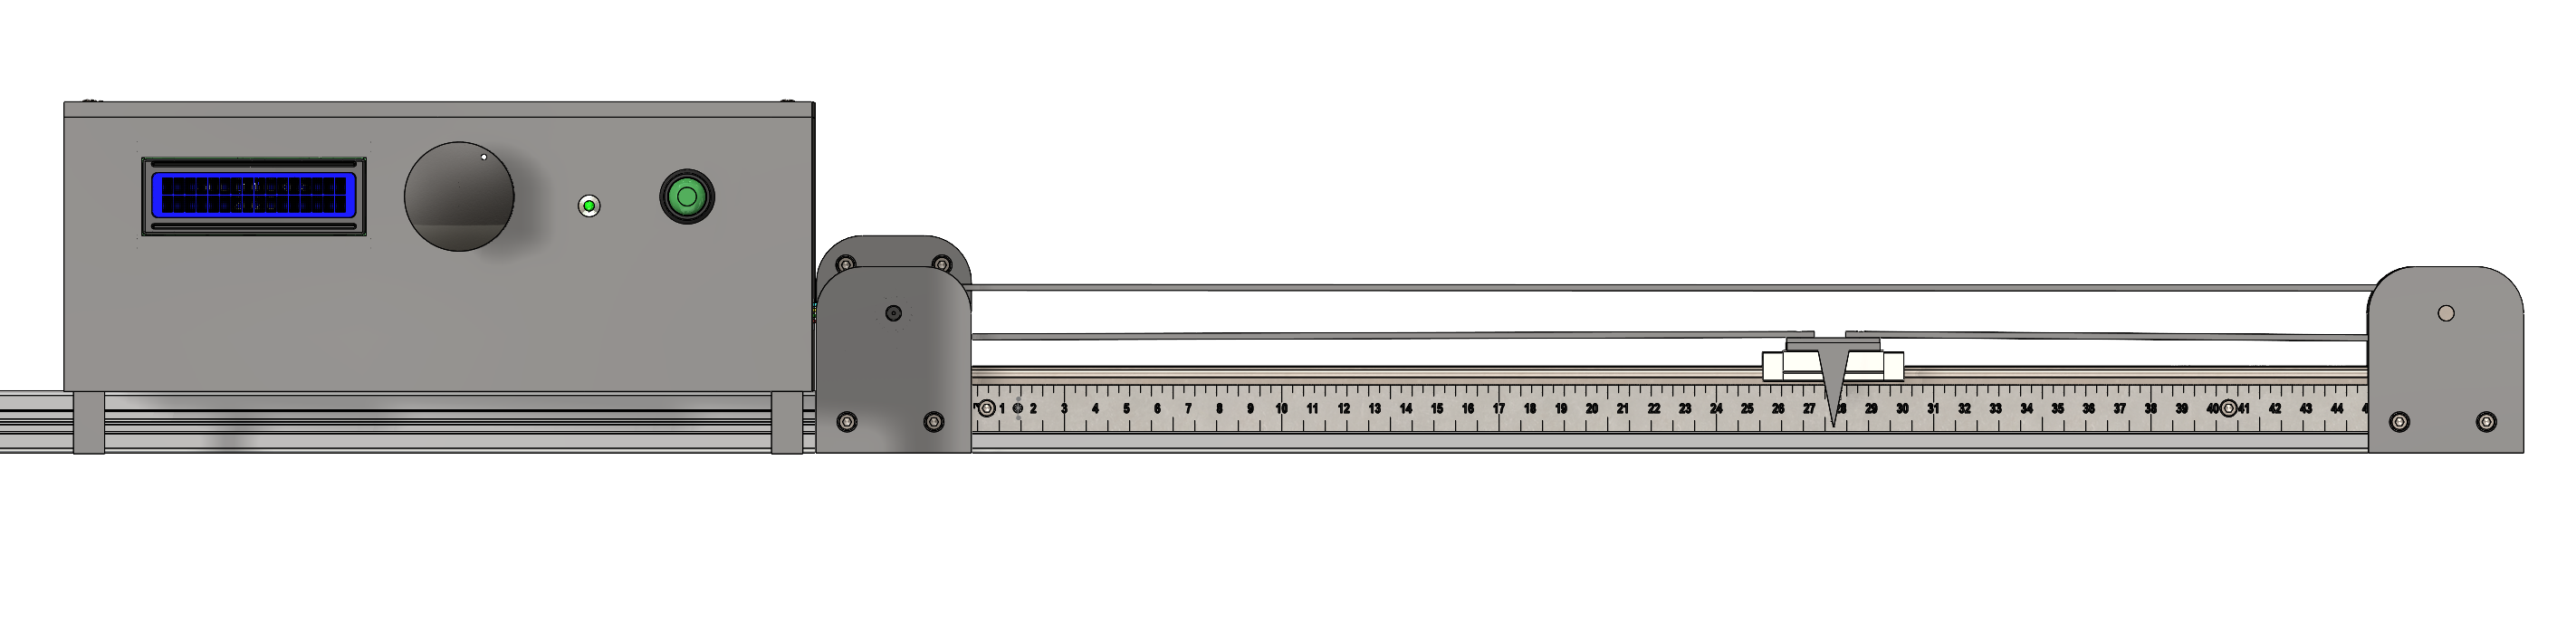
\includegraphics[width=\textwidth]{Images/Konstruktion1.png}
		\caption{CAD-Modell (Eigenaufnahme)} \label{CADMOD}
	\end{center}
\end{figure} 

\begin{figure}[H]
	\begin{center}
		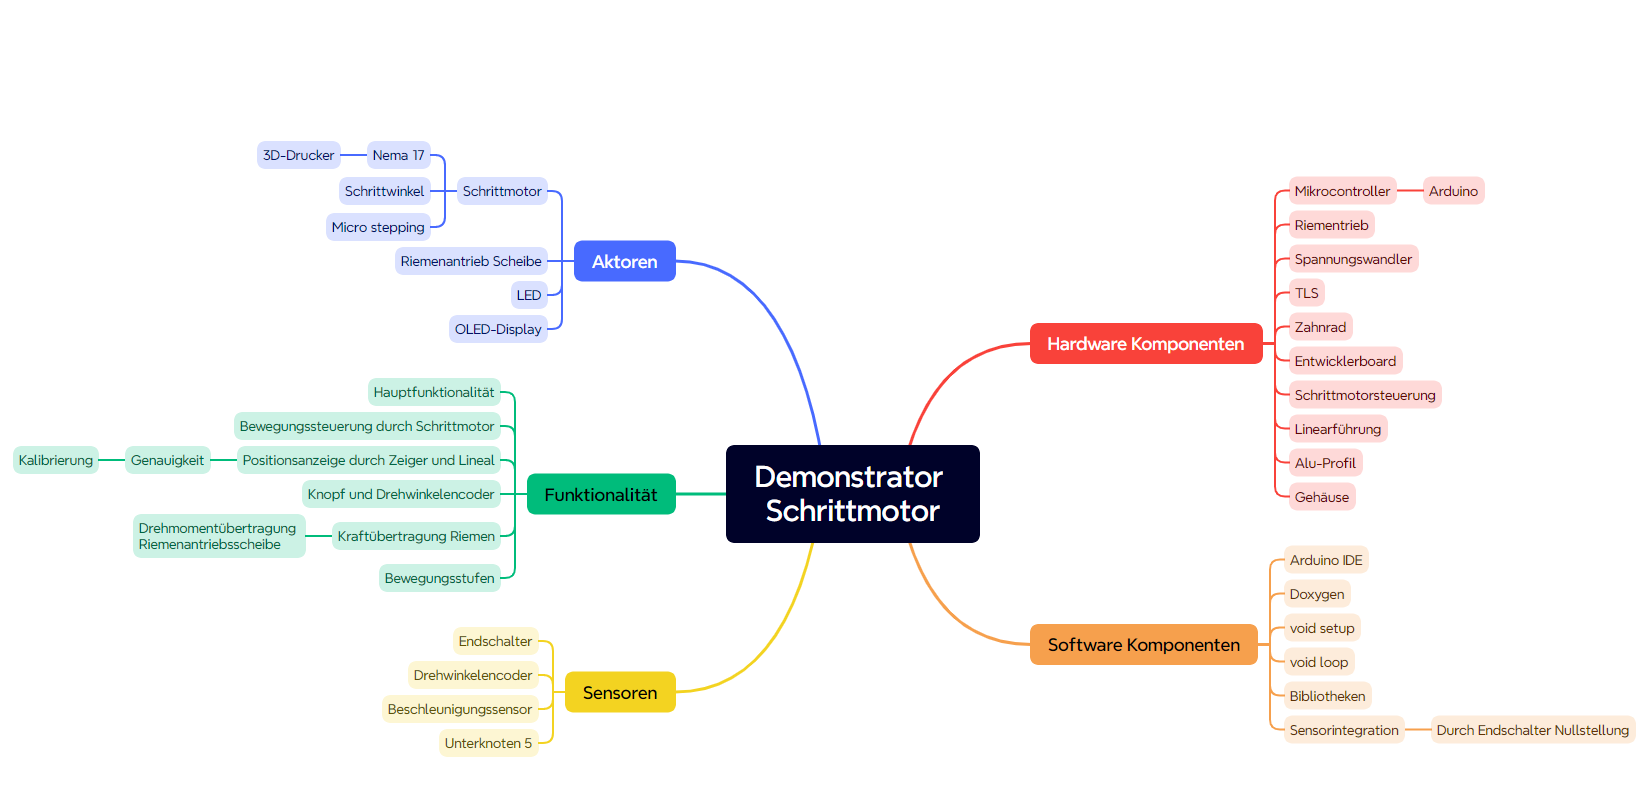
\includegraphics[width=\textwidth]{../Appendix/Mindmap/Mindmap.png}
		\caption{Mindmap} \label{Mindmap}
	\end{center}
\end{figure} 

\section{Anwendungsbereich des Demonstrators}

Die grundsätzliche Aufgabe des Demonstrators ist es, die Funktionsweise eines Schrittmotors zu veranschaulichen. Der Demonstrator soll zur Veranschaulichung und als ergänzendes Lehrmittel dienen. So können Studierende die Prinzipien der Schrittmotorsteuerung einschließlich Schrittauflösung und Positionierung praxisnah erlernen. Darüber hinaus können die Studierenden den Demonstrator nutzen, um praktische Erfahrungen zu sammeln, z.B. durch Programmierübungen. Darüber hinaus könnte ein solcher Demonstrator als Qualitätskontrolle dienen, um die Leistungsfähigkeit und Genauigkeit von Schrittmotoren zu überprüfen und sicherzustellen, dass diese den geforderten Spezifikationen entsprechen. Ein weiteres Anwendungsgebiet können Fachmessen sein, um mit einem solchen Demonstrator Bewegungsabläufe und Positioniergenauigkeit zu demonstrieren.  

\section{Besondere Herausforderungen bei den Quellen}

Die größte Herausforderung bei der Beschaffung von Literaturquellen ist die Sprachbarriere, wenn relevante Quellen nur in Englisch oder anderen Sprachen verfügbar sind. Diese Barriere kann das Verständnis und die Interpretation der Quellen erheblich erschweren. Dies führt zu erhöhtem Aufwand, da Quellen häufig übersetzt werden müssen. Online-Tools wie Deepl (\href{https://www.deepl.com/de/translator}{www.deepl.com}) können hier Abhilfe schaffen. Ein weiteres Problem ist die mangelnde Verfügbarkeit von Datenblättern, die von den Herstellern trotz mehrfacher Nachfrage nicht zur Verfügung gestellt wurden. Datenblätter sind für technische Projekte unerlässlich, da sie wichtige Informationen über die Funktionsweise und die Einsatzmöglichkeiten liefern. Ein weiteres Problem ist das Fehlen des Veröffentlichungsdatums oder die Veralterung der Quellen. Dies erschwert eine genaue Dokumentation, da der aktuelle Stand der Technik nicht genau nachvollzogen werden kann. 